\subsection*{Binomials}
\begin{align*}
\sum_{k = 0}^{n} C_n^k &= 2^n &
\sum_{k = 0}^{m} C_{n + k}^k &= C_{n + m + 1}^m \\
\sum_{m = 0}^{n} C_m^k &= C_{n + 1}^{k + 1} &
\sum_{k = 0}^{n} (C_n^k)^2 &= C_{2n}^n \\
\sum_{j = 0}^{k} C_m^j C_{n-m}^{k - j} &= C_n^k &
\sum_{j = 0}^{m} C_m^j C_{n-m}^{k - j} &= C_{n + 1}^{k + 1} \\
\sum_{k = 0}^{n} C_{n - k}^k &= F_{n + 1} &&
\end{align*}

\subsection*{Catalan numbers}
$$C_n = \sum_{k = 0}^{n - 1} C_kC_{n - 1 - k} = \frac{1}{n + 1} C_{2n}^{n} = C_{2n}^{n} - C_{2n}^{n - 1}$$

1, 1, 2, 5, 14, 42, 132, 429, 1430, 4862, 16796, 58786


\subsection*{Fibonacci numbers}
\begin{align*}
F_1 &= F_2 = 1 &
\text{gcd}(F_m, F_n) &= F_{\text{gcd}(n, m)} \\
F_n &= F_{n - 1} + F_{n - 2} &
F_{n + 1} F_{n - 1} - F_n^2 &= (-1)^n \\
F_{n + k} &= F_k F_{n + 1} + F_{k - 1} F_n &
F_{47} &\approx 2.9 \cdot 10^9\\
F_n &= \frac{(\tfrac{1 + \sqrt{5}}{2})^n - (\tfrac{1 - \sqrt{5}}{2})^n}{\sqrt{5}} &
F_{88} &\approx 1.1 \cdot 10^{18}
\end{align*}

\subsection*{Stirling numbers of the second kind}

$S(n, k)$ – the number of ways to divide $n$ element into $k$ non-empty groups.\\

$S(n, n) = 1$, $n \ge 0$

$S(n, 0) = 0$, $n > 0$

$S(n, k) = S(n - 1, k - 1) + S(n - 1, k) \cdot k$.

$B_n = \sum_{k=0}^n S(n, k)$ from $n = 0$:

1, 1, 2, 5, 15, 52, 203, 877, 4140, 21147, 115975, 678570, 4213597, 27644437, 190899322, 1382958545, 10480142147, 82864869804,...

\subsection*{Generating functions}
$$[x^i](1 + x)^n = C_{n}^{i} \quad [x^i](1 - x)^{-n} = C_{n + i - 1}^{i}$$

$$C_{\alpha}^n = \frac{\alpha(\alpha - 1) \dots (\alpha - n + 1)}{n!}$$

$$\prod_{n = 1}^\infty (1 - x^n) = \sum_{k = -\infty}^{\infty} (-1)^k x^{\frac{k(3k - 1)}{2}} \text{(pentagonal number theorem)}$$

\subsection*{Hook length formula}

\begin{wrapfigure}{r}{0.1\textwidth}
    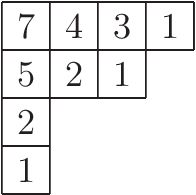
\includegraphics[width=\linewidth]{content/mathematics/hook-length-tableau.jpg}
    A tableau listing the hook length of each cell in the Young diagram $(4, 3, 1, 1)$
\end{wrapfigure}

A standard Young tableau is a filling of the $n$ cells of the Young diagram with a permutation, 
such that each row and each column form increasing sequences. 
The \textbf{hook} $h_{\lambda}(i, j)$ is number of cells $(a, b)$ in diagram such that
$a = i$ and $b \ge j$ or $a \ge i$ and $b = j$.

The number of standard Young tableaux of shape $\lambda$:
$$f^\lambda = \frac{n!}{\prod h_{\lambda}(i, j)}$$


\subsection*{Burnside's lemma}

Let $G$ be a finite group that acts on a set $X$.

The \textit{orbit} of an element $x$ in $X$ is the set of elements
in $X$ to which $x$ can be moved by the elements of $G$.
The orbit of $x$ is denoted by $G \cdot x$:
 $$G \cdot x = \{g \cdot x\, |\, g \in G\}.$$
For each $g$ in $G$, let $X^g$ denote the set of elements
in $X$ that are fixed by $g$ (also said to be left invariant by $g$),
that is, $X^g = \{ x \in X\, |\, g \cdot x = x \}$.
Burnside's lemma asserts the following formula for the number of orbits,
denoted $|X/G|$:
$$|X/G| = \frac{1}{|G|} \sum_{g \in G} |X^g|.$$
